\begin{figure}[H]
    \centering
    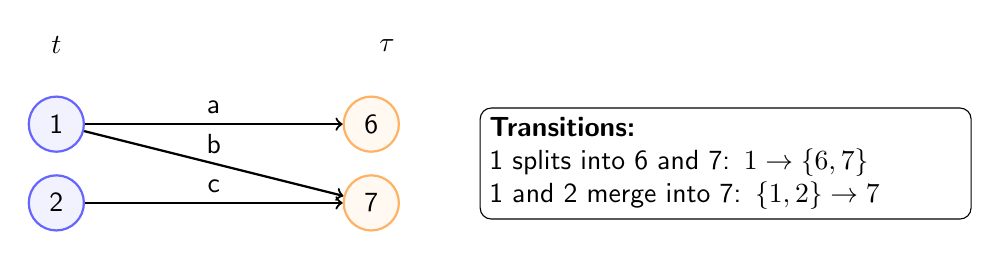
\begin{tikzpicture}[
            leftnode/.style={circle, draw=blue!60, fill=blue!5, thick, minimum size=7mm},
            rightnode/.style={circle, draw=orange!60, fill=orange!5, thick, minimum size=7mm},
            font=\sffamily,
            node distance=8mm and 30mm
        ]

        % Time labels
        \node[font=\bfseries] at (0,2) {$t$};
        \node[font=\bfseries] at (4.2,2) {$\tau$};

        % Left nodes
        \node[leftnode] (n1) at (0,1) {1};
        \node[leftnode] (n2) at (0,0) {2};

        % Right nodes
        \node[rightnode] (n6) at (4,1) {6};
        \node[rightnode] (n7) at (4,0) {7};

        % Edges
        \draw[->, thick] (n1) -- (n6) node[midway, above] {a};
        \draw[->, thick] (n1) -- (n7) node[midway, above] {b};
        \draw[->, thick] (n2) -- (n7) node[midway, above] {c};

        % Legend (left)
        \node[align=left, anchor=center, text width=6cm, draw, rounded corners] (legend) at (8.5,0.5) {
            \textbf{Transitions:} \\
            1 splits into 6 and 7: $1 \rightarrow \{6, 7\}$ \\
            1 and 2 merge into 7: $\{1, 2\} \rightarrow 7$
        };

    \end{tikzpicture}

    \vspace{1em}

    % Table below the diagram
    \begin{minipage}{0.8\textwidth}
        \centering
        \begin{tabular}{|c|c|c|l|}
            \hline
            \textbf{Edge} & \textbf{From} & \textbf{To} & \textbf{Transition Type} \\
            \hline
            a             & 1             & 6           & Split                    \\
            b             & 1             & 7           & Mergesplit               \\
            c             & 2             & 7           & Merge                    \\
            \hline
        \end{tabular}
    \end{minipage}
    \caption{Example of a mergesplit transition.}
    \label{fig:cluster-mergesplit}
\end{figure}